\documentclass[8pt]{beamer}

\usepackage{verse}
\usepackage{graphicx}

\usetheme{metropolis}

\setbeamersize{text margin left=5pt,text margin right=5pt}

\begin{document}

\begin{frame}
	\frametitle{West-Kap}
	\begin{figure}[H]
		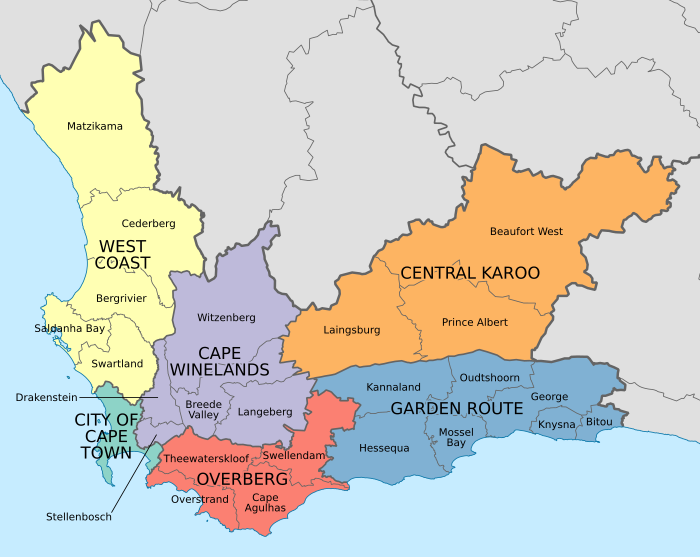
\includegraphics[scale=0.3]{western_cape}
	\end{figure}
\end{frame}

\begin{frame}
	\frametitle{Winter: Boland}
	\begin{figure}[H]
		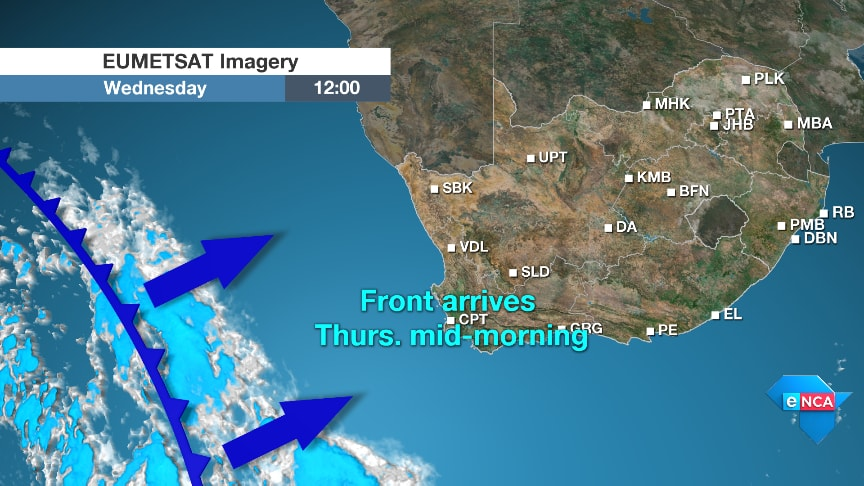
\includegraphics[scale=0.3]{front}
	\end{figure}
\end{frame}

\begin{frame}
	\frametitle{Winter: Boland}
	\begin{figure}[H]
		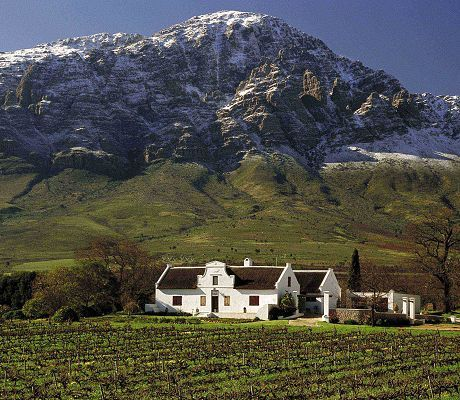
\includegraphics[scale=0.6]{wynland}
	\end{figure}
\end{frame}

\begin{frame}
	\frametitle{Vroegherfs (N.P. van Wyk Louw)}
	\begin{center}
		\settowidth{\versewidth}{laat ryp word, Heer, laat u wind waai,
		laat stort }
		\begin{minipage}[t]{\dimexpr\versewidth+1sp\relax}
			\begin{verse}[\versewidth]
				Die jaar word ryp in goue akkerblare, \\
				in wingerd wat verbruin, en witter lug \\
				wat daglank van die nuwe wind en klare \\
				son deurspoel word; elke blom word vrug, \\
				tot selfs die traagstes; en die eerste blare val
				\\
				so stilweg in die rook-vaal bos en laan, \\
				dat die takke van die lang populiere al \\
				teen elke ligte m{\^o}re witter staan. \\
				O Heer, laat hierdie dae heilig word: \\
				laat alles val wat pronk en sieraad was \\
				of enkel jeug, en v{\'e}r was van die pyn; \\
				laat ryp word, Heer, laat u wind waai, laat
				stort \\
				my waan, tot al die hoogheid eindelik vas \\
				en nakend uit my teerder jeug verskyn.
			\end{verse}
		\end{minipage}\hfill
		\settowidth{\versewidth}{laat ryp word, Heer, laat u wind waai,
		laat stort}
		\begin{minipage}[t]{\dimexpr\versewidth+1sp\relax}
			\begin{verse}[\versewidth]
				Das Jahr reift zu goldenen Eichelbl{\"a}ttern,
				\\
				in einem Weinberg, der br{\"a}unt, und
				wei{\ss}ere Luft \\
				die den ganzen Tag von dem neuen Wind und klarer
				\\
				Sonne gesp{\"u}lt wird; jeder Blume wird Frucht,
				\\
				selbst die langsamsten; und die ersten
				Bl{\"a}tter fallen \\
				so leise im rauch-blassen Wald und Allee, \\
				dass die Zweige der langen Pappeln immer \\
				an jedem hellen Morgen wei{\ss}er stehen. \\
				O Herr, lass diese Tage geheiligt sein: \\
				Lass alles fallen, was Angeberei und Schmuck
				war \\
				oder nur Jugend und weit vom Schmerz entfernt;
				\\
				Lass es reifen, Herr, lass deinen Wind wehen,
				lass meinen Wahn \\
				fallen , biss alle Hoheit endlich fest
				\\
				und nackt aus meiner zarten Jugend erscheint .
			\end{verse}
		\end{minipage}
	\end{center}
\end{frame}

\end{document}
